\fenicschapter{Block preconditioning of systems of PDEs}
              {Block preconditioning of systems of PDEs}
              {Kent-Andre Mardal and Joachim Berdal Haga}
              {mardal-4}

\newcommand{\algorithmexample}[3]{%
\begin{figure*}
  \begin{center}
    \small
    \begin{tabular}{l}
      \hline
      \textbf{Algorithm example #1:} #2 \\
      \hline
      \begin{minipage}{0.9\textwidth}
        \vspace{0.1cm}
        \begin{enumerate}
          #3
        \end{enumerate}
        \vspace{0.1cm}
      \end{minipage} \\
      \hline
    \end{tabular}
    \normalsize
  \end{center}
\end{figure*}}

In this chapter we describe the implementation of block preconditioned
Krylov solvers for systems of partial differential equations (PDEs)
using \emp{cbc.block}\index{\emp{cbc.block}} and the Python interfaces of
DOLFIN and Trilinos\index{Trilinos}.  We start by reviewing the
abstract theory of constructing preconditioners\index{preconditioner}
by considering the differential operators as mappings in properly
chosen Sobolev spaces, before giving a short overview
of \emp{cbc.block}. We then present several examples, namely the
Poisson problem, the Stokes problem, the time-dependent Stokes problem
and finally a mixed formulation of the Hodge Laplacian.

\section{Abstract framework for constructing preconditioners}

This presentation of preconditioning is largely taken from the review
paper~\citep{MardalWinther11}, where a more comprehensive mathematical
presentation is given. Consider the following abstract formulation of
a linear PDE problem: Find $u$ in a Hilbert space $H$ such that:
\begin{equation}
\mathcal{A} u = f,
\end{equation}
where $f\in H'$ and $H'$ is the dual space of $H$.
We will assume that the PDE problem is well-posed; that is,
$\mathcal{A} : H \rightarrow H'$ is a bounded invertible operator in the sense that,
\begin{equation}
\|\mathcal{A}\|_{\mathcal{L} (H, H')} \le C \quad \mbox{and} \quad
\|\mathcal{A}^{-1}\|_{\mathcal{L} (H', H)} \le C.
\end{equation}
The reader should notice that this operator is bounded only when
viewed as an operator from $H$ to $H'$.  The spectrum of the operator
is unbounded and discretizations of the operator will typically have
condition numbers that increase in negative powers of $h$, where $h$
is the characteristic cell size, as the mesh is refined.  The remedy
for the unbounded spectrum is to introduce a preconditioner.  Let the
preconditioner $B$ be an operator mapping $H'$ to $H$ such that
\begin{equation}
\|\mathcal{B}\|_{\mathcal{L}(H', H)} \le C \quad \mbox{and} \quad
\|\mathcal{B}^{-1}\|_{\mathcal{L}(H, H')} \le C.
\end{equation}
Then
$\mathcal{B}\mathcal{A}: H \rightarrow H$ and
\begin{equation}
\|\mathcal{B}\mathcal{A}\|_{\mathcal{L}(H, H)} \le C^2 \quad \mbox{and} \quad
\|(\mathcal{B}\mathcal{A})^{-1}\|_{\mathcal{L}(H, H)} \le C^2.
\end{equation}
Hence, the spectrum and therefore the condition number of the
preconditioned operator is bounded:
\begin{equation}
  \kappa(\mathcal{B}\mathcal{A}) = \|\mathcal{B}\mathcal{A}\|_{\mathcal{L}(H, H)} \|(\mathcal{B}\mathcal{A})^{-1}\|_{\mathcal{L}(H, H)} \le C^4.
\end{equation}
One example of such a preconditioner is the Riesz operator
$\mathcal{R}$; that is, the identity mapping between $H'$ and $H$.  In
this case
\begin{equation}
\|\mathcal{R}\|_{\mathcal{L}(H', H)} = 1 \quad \mbox{and} \quad
\|\mathcal{R}^{-1}\|_{\mathcal{L}(H, H')} = 1.
\end{equation}
In fact, in most of our examples the preconditioners are approximate Riesz mappings.

Given that the discretized operators  $\mathcal{A}_h$ and $\mathcal{B}_h$ are stable; that is,
 \begin{equation}
\|\mathcal{A}_h\|_{\mathcal{L} (H, H')} \le C, \ \|\mathcal{A}_h^{-1}\|_{\mathcal{L} (H', H)} \le C, \
\|\mathcal{B}_h\|_{\mathcal{L}(H', H)} \le C,  \  \|\mathcal{B}_h^{-1}\|_{\mathcal{L}(H, H')} \le C,
\end{equation}
then the condition number of the discrete preconditioned operator,
$\kappa(\mathcal{B}_h \mathcal{A}_h)$, will be bounded by $C^4$
independently of $h$.  Furthermore, the number of iterations required
by a Krylov solver to reach a certain convergence criterion can
typically be bounded by the condition number. Hence, when the
condition number of the discrete problem is bounded independent of
$h$, the Krylov solvers will have a convergence rate that is
independent of $h$.  If $\mathcal{B}_h$ is similar to $\mathcal{A}_h$
in terms of storage and evaluation, then the solution algorithm
is \emph{order-optimal}.  We remark that it is crucial that
$\mathcal{A}_h$ is a stable operator and we will illustrate what
happens for unstable operators in the example concerning Stokes
problem.  Finally, we will see that $\mathcal{B}_h$ often can be
constructed using multigrid techniques. These multigrid
preconditioners will be spectrally equivalent with the Riesz mappings.

\section{Overview of \emp{cbc.block}}

\emp{cbc.block} makes it possible to write matrix operations in mathematical notation, such as $M = A B+C$, where $A$, $B$ and $C$ are matrices or operators. The algebraic operations are not performed explicitly; instead the operators are stored in a graph as shown in Figure~\ref{fig:mardal-4:block:dag}. When $M$ is called upon to operate on a vector, as in $y=Mx$, the individual operations are performed in the right order on the vector: $u=Bx$, $v=Au$, $w=Cx$, $y=v+w$. Since the matrix product or sum is not created explicitly, the individual operators do not need to have an explicit matrix representation, but  may be a DOLFIN matrix, a preconditioner such as ML, or even an inner iterative solver.
To enable the construction of this graph \emp{cbc.block} injects the
methods \emp{\_\_mul\_\_}, \emp{\_\_add\_\_}, and \emp{\_\_sub\_\_}
into the \emp{Matrix} and \emp{Vector} classes in \dolfin.  The module
also implements block partitioned matrices and vectors. These are pure
python objects, and do not use the block matrix in \dolfin.

%\begin{figure}
%%\centering
%\def\svgwidth{\largefig}
%%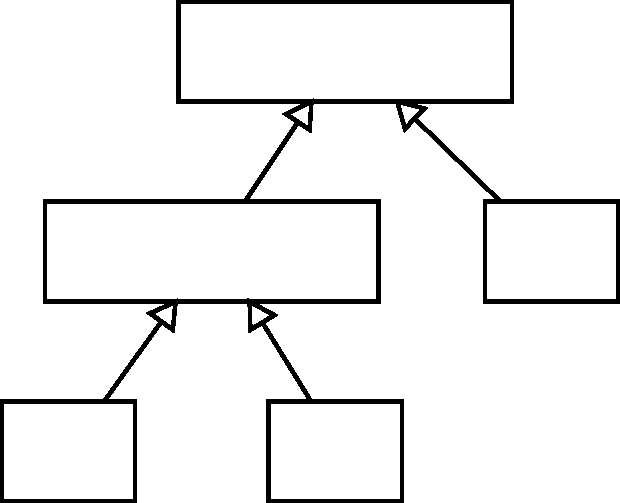
\includegraphics[width=\largefig]{chapters/mardal-4/pdf/block.pdf}
%\import{chapters/mardal-4/pdf/}{block.pdf_tex}
%\caption{Expression tree for the composed matrix $M = A B + C$.}
%\label{block:dag}
%\end{figure}
%
\begin{figure}
  \center\fenicsfig{mardal-4}{block}{\largefig}
  \caption{Expression tree for the composed matrix $M = A B + C$.}
  \label{fig:mardal-4:block:dag}
\end{figure}

When the explicit matrix product is required, such as for input to the
ML preconditioner, a method \emp{collapse} is provided that performs
the calculations using PyTrilinos. This method requires that all
components are actual matrices, not general operators.

The module also provides services to set Dirichlet boundary conditions
and perform other transformations of the system, and a range of
iterative solvers and preconditioners.

\section{Numerical examples}

In all examples the mesh will be refinements of the unit square or
unit cube.  The code examples presented in this chapter differ
slightly from the source code, in the sense that import statements,
safety checks, command-line arguments, definitions of \emp{Functions}
and \emp{Subdomains} are often removed to shorten the presentation.

\subsection{The Poisson problem with homogeneous Neumann conditions}
The Poisson equation with Neumann conditions reads:
Find $u$ such that
\begin{align}
  -\Delta u &= f \mbox{ in } \Omega,  \\
  \frac{\partial u}{\partial n} &= g \mbox{ on } \partial \Omega .
\end{align}
The corresponding variational problem is:  Find $u\in H^1 \cap L^2_0$ such that
\[
\int_\Omega \nabla u \cdot \nabla v \dx = \int_\Omega f v \dx +
\int_{\partial \Omega} g v  \ds, \quad\foralls v \in H^1 \cap L^2_0 .
\]
Let the linear operator $\mathcal{A}$ be defined in terms of the  bilinear form,
\[
(\mathcal{A} u, v) =  \int_\Omega \nabla u \cdot \nabla v \dx.
\]
It is well-known that $\mathcal{A}$ is a bounded invertible operator
from $H^1 \cap L^2_0$ into its dual space.  Furthermore, it is
well-known that one can construct multigrid preconditioners for this
operator such that the preconditioner is spectrally equivalent with
the inverse of $\mathcal{A}$, independent of the characteristic size
of the cells in the
mesh~\citep{Bramble1993,Hackbusch1994,TrottenbergOosterleeSchuller2001}.

In this example, we use a multigrid preconditioner based on the
algebraic multigrid package ML contained in
PyTrilinos\index{PyTrilinos}. Furthermore, we will estimate the
eigenvalues of the preconditioned system. We use continuous piecewise
linear elements and compute the condition number of the preconditioned
system and corresponding number of iteration required for convergence
using the conjugate gradient method\index{conjugate gradient method}
for various uniform refinements of the unit square.

First of all, the ML preconditioner is constructed as follows,
\begin{python}
class ML(block_base):
    def __init__(self, A, pdes=1):
        # create the ML preconditioner
        MLList = {
            "smoother: type"            : "ML symmetric Gauss-Seidel" ,
            "aggregation: type"         : "Uncoupled" ,
            "ML validate parameter list": True,
            }
        self.A = A # Prevent matrix being deleted
        self.ml_prec = MultiLevelPreconditioner(A.down_cast().mat(), 0)
        self.ml_prec.SetParameterList(MLList)
        self.ml_agg = self.ml_prec.GetML_Aggregate()
        self.ml_prec.ComputePreconditioner()

    def matvec(self, b):
        x = self.A.create_vec()
        self.ml_prec.ApplyInverse(b.down_cast().vec(), x.down_cast().vec())
        return x
\end{python}
The linear algebra backends uBLAS, PETSc and Trilinos all have a wide
range of Krylov solvers. Here, we implement these solvers in Python
because we need to store intermediate variables and used them to
compute an estimate of the condition number.  The following code shows
the implementation of the conjugate gradient method using the Python
linear algebra interface in DOLFIN:
\begin{python}
def precondconjgrad(B, A, x, b, tolerance, maxiter, progress, relativeconv=False):

    r = b - A*x
    z = B*r
    d = z
    rz = inner(r,z)

    iter = 0
    alphas = []
    betas = []
    residuals = [sqrt(rz)]

    if relativeconv:
        tolerance *= residuals[0]

    while residuals[-1] > tolerance and iter <= maxiter:
        z = A*d
        dz = inner(d,z)
        alpha = rz/dz
        x += alpha*d
        r -= alpha*z
        z = B*r
        rz_prev = rz
        rz = inner(r,z)
        beta = rz/rz_prev
        d = z + beta*d

        iter += 1
        progress += 1
        alphas.append(alpha)
        betas.append(beta)
        residuals.append(sqrt(rz))

    return x, residuals, alphas, betas
\end{python}
The intermediate variables called alphas and betas can then be used to
estimate the condition number of the preconditioned matrix as follows;
see~\citet{Saad2003}.  Notice that since the preconditioned
conjugate gradient method converges quite fast when using algebraic
multigrid (AMG)\index{AMG} as a preconditioner, there will be only a
small number of alphas and betas. Therefore we use the dense linear
algebra tools in NumPy to compute the eigenvalue estimates.
\begin{python}
    def eigenvalue_estimates(self):
        # eigenvalues estimates in terms of alphas and betas

        import numpy

        n = len(self.alphas)
        M = numpy.zeros([n,n])
        M[0,0] = 1/self.alphas[0]
        for k in range(1, n):
            M[k,k] = 1/self.alphas[k] + self.betas[k-1]/self.alphas[k-1]
            M[k,k-1] = numpy.sqrt(self.betas[k-1])/self.alphas[k-1]
            M[k-1,k] = M[k,k-1]
        e,v = numpy.linalg.eig(M)
        e.sort()
        return e
\end{python}
The following code shows the implementation of a Poisson problem
solver, using the above mentioned ML preconditioner and conjugate
gradient algorithm. We remark here that it is essential for the
convergence of the method that both the start vector and the
right-hand side are both in $L^2_0$. For this reason we subtract the
mean value from the right hand-side.  The start vector is zero and
does therefore have mean value zero.
\begin{python}
# Create mesh and finite element
mesh = UnitSquare(N,N)
V = FunctionSpace(mesh, "CG", 1)

# Define variational problem
v = TestFunction(V)
u = TrialFunction(V)
f = Source()
g = Flux()

a = dot(grad(v), grad(u))*dx
L = v*f*dx + v*g*ds

# Assemble matrix and vector
A, b = assemble_system(a,L)

# remove constant from right handside
c = b.array()
c -= sum(c)/len(c)
b[:] = c

# create preconditioner
B = ML(A)
Ainv = ConjGrad(A, precond=B, tolerance=1e-8)

x = Ainv*b

e = Ainv.eigenvalue_estimates()

print "N=%d iter=%d K=%.3g" % (N, Ainv.iterations, e[-1]/e[0])
\end{python}
In Table~\ref{tabel:neumann} we list the number of iterations for
convergence and the estimated condition number of the preconditioned
system based on the code shown above. We test different
refinements of the unit square and continuous piecewise linear
elements, $\mathrm{CG}_1$. The source function is $f=
500\exp(-((x-0.5)^2 + (y-0.5)^2)/0.02)$ and the boundary condition is
$g = 25 \sin(5\pi y)$ for $x=0$ and zero elsewhere, see also the
source code \emp{poisson\_neumann.py}.
\begin{table}
\begin{center}
\begin{tabular}{|c||c|c|c|c|c|c|}
\hline
$h$ & $2^{-4}$ & $2^{-5}$ & $2^{-6}$ & $2^{-7}$ & $2^{-8}$ \\ \hline \hline
$\kappa$ & 1.57 & 1.26 & 2.09 & 1.49 & 1.20 \\ \hline
$\#iterations$ & 8 & 8 & 10 & 9 & 7 \\ \hline
\end{tabular}
\caption{The estimated condition number $\kappa$ and the number of iterations for
  convergence with respect to various uniform mesh refinements for the Poisson
  problem with Neumann conditions solved with the
  $\mathrm{CG}_1$ method.}\label{tabel:neumann}
\end{center}
\end{table}

\subsection{The Stokes problem}
Our next example is the Stokes problem,
\begin{align}
  -\Delta u - \nabla p &= f \quad \mbox{in} \ \Omega, \\
  \nabla \cdot u &= 0 \quad \mbox{in} \  \Omega, \\
  u &= g   \quad \mbox{on} \  \partial \Omega.
\end{align}
The variational form is: \\
Find $u,p \in H^1_g \times L_0^2$ such that
\[
\int_\Omega \nabla u : \nabla v \dx +
\int_\Omega \nabla \cdot u \, q \dx +
\int_\Omega \nabla \cdot v \, p \dx = \int_\Omega f\, v \dx   , \quad
\foralls v,q \in H^1_0 \times L_0^2.
\]
Let the linear operator $\mathcal{A}$ be defined as
\[
\mathcal{A}  =
\begin{pmatrix} A & B^* \\ B & 0 \end{pmatrix}.
\]
where
\begin{align}
  (A u, v) &= \int_\Omega \nabla u : \nabla v \dx, \\
  (B u, q) &= \int_\Omega \nabla \cdot u \, q \dx,
\end{align}
and $B^*$ is the adjoint of $B$.  Then it is well-known that
$\mathcal{A}$ is a bounded operator from $H^1_g \times L_0^2$ to its
dual $H_g^{-1} \times L_0^2$, see for
example~\citet{Brezzi1974,BrezziFortin1991}. Therefore, we construct a
preconditioner, $\mathcal{B}: H_g^{-1} \times L_0^2 \rightarrow
H^1_g \times L_0^2$ defined as
\[
\mathcal{B}
=
\begin{pmatrix} K^{-1} & 0 \\ 0 & L^{-1} \end{pmatrix}.
\]
where
\begin{align}
  (K u, v) &= \int_\Omega \nabla u: \nabla v \dx, \\
  (L p, q) &= \int_\Omega p \, q \dx.
\end{align}
We refer to \citet{MardalWinther11} for a mathematical explanation of
the derivation of such preconditioners.  Notice that the operator
$\mathcal{B}$ is positive in contrast to $\mathcal{A}$. Hence, the
preconditioned operator $\mathcal{B} \mathcal{A}$ will be
indefinite. For both $K$ and $L$, we use the AMG preconditioner
provided by ML/Trilinos as described in the previous example (A simple
Jacobi preconditioner would be sufficient for $L$).  For symmetric
indefinite problems the \emph{Minimum Residual Method} is the fastest
method. Preconditioners of this form has been studied by
many~\citep{ElmanSilvesterWathen2005,RustenWinther1992,SilvesterWathen1993,SilvesterWathen1994}.

In Table~\ref{stokes:ex} we present the number of iterations needed
for convergence and estimates on the condition number $\kappa$ with
respect to different discretization methods and different
characteristic cell sizes $h$. The problem we are solving is the
so-called lid driven cavity problem; that is, $f=0$ and $g = (1,0)$ for
$y=1$ and zero elsewhere.  We use different mixed methods, namely the
$\mathrm{CG}_2-\mathrm{CG}_1$, $\mathrm{CG}_2-\mathrm{DG}_0$,
$\mathrm{CG}_1-\mathrm{CG}_1$, and $\mathrm{CG}_1-\mathrm{CG}_1$
stabilized.  The iteration is stopped when $(\mathcal{B}_h r_k,
r_k)/(\mathcal{B}_h r_0, r_0) \le 10^{-8}$, where $r_k$ is the
residual at iteration $k$.  The condition numbers, $\kappa$, were
estimated using the conjugate gradient method on the normal
equation. This condition number will always be less than the real
condition number and is probably too low for the last columns for the
$\mathrm{CG}_1-\mathrm{CG}_1$ method without stabilization.
Notice that for the stable methods that satisfy the
LBB condition (see also Chapter~\ref{chap:rognes}); that is,
\index{Ladyzhenskaya--\babuska{}--Brezzi conditions}
\index{LBB conditions}
 $\mathrm{CG}_2-\mathrm{CG}_1$
and $\mathrm{CG}_2-\mathrm{DG}_0$, the number of iterations and the
condition number seems to be bounded independently of $h$. For the
unstable $\mathrm{CG}_1-\mathrm{CG}_1$ method, the number of
iterations and the condition number increases as $h$
decreases, but is here stopped. However, for the stabilized method,
$\mathrm{CG}_1-\mathrm{CG}_1$-stab, where the pressure is stabilized
by
\[
\int_\Omega \nabla \cdot u \, q  - \alpha h^2 \, \nabla p \cdot \nabla q
    \dx,
\]
with $\alpha=0.01$, the number of iterations and the condition number appear to be bounded.

\begin{table}
\begin{center}
\begin{tabular}{|c|c||c|c|c|c|c|c|}
\hline
method & $h$ & $2^{-4}$ & $2^{-5}$ & $2^{-6}$ & $2^{-7}$ & $2^{-8}$ \\ \hline\hline
$\mathrm{CG}_2-\mathrm{CG}_1$ &  iterations & 52 & 57 & 62 & 64 & 67 \\ \hline
$\mathrm{CG}_2-\mathrm{CG}_1$ & $\kappa $ & 13.6 & 13.6 & 13.6 & 13.6 & 13.6 \\ \hline
$\mathrm{CG}_2-\mathrm{DG}_0$ &  iterations & 43 & 48 & 55 & 59 & 62 \\ \hline
$\mathrm{CG}_2-\mathrm{DG}_0$ & $\kappa $ & 8.5 & 9.2 & 9.7 & 10.3 & 10.7 \\ \hline
$\mathrm{CG}_1-\mathrm{CG}_1$ & iterations & 200+ & 200+ & 200+ & 200+ & 200+ \\ \hline
$\mathrm{CG}_1-\mathrm{CG}_1$ & $\kappa$ & 696 & 828 & 672 & 651 & 630 \\ \hline
$\mathrm{CG}_1-\mathrm{CG}_1$-stab& iterations & 41 & 40 & 40 & 39 & 39 \\ \hline
$\mathrm{CG}_1-\mathrm{CG}_1$-stab& $\kappa $ & 12.5 & 12.6 & 12.7 & 12.7 & 12.7 \\ \hline
\end{tabular}
\caption{Estimated condition number $\kappa$ and number of iterations for
  convergence with respect to mesh refinements.
  The methods $\mathrm{CG}_2-\mathrm{CG}_1$, $\mathrm{CG}_2-\mathrm{DG}_0$, and $\mathrm{CG}_1-\mathrm{CG}_1$-stab are stable, while $\mathrm{CG}_1-\mathrm{CG}_1$ is not.}\label{stokes:ex}
\end{center}
\end{table}

We will now describe the code in detail.  In this case, the
preconditioner consists of two preconditioners.  The following shows
how to implement this block preconditioner\index{block preconditioner}
based on the ML preconditioner defined in the previous example.
\begin{python}
mesh = UnitSquare(N,N)
def CG(n):
    return ('DG',0) if n==0 else ('CG',n)

V = VectorFunctionSpace(mesh, *CG(vorder))
Q = FunctionSpace(mesh, *CG(porder))

f = Constant((0,0))
g = Constant(0)
alpha = Constant(alpha)
h = CellSize(mesh)

v,u = TestFunction(V), TrialFunction(V)
q,p = TestFunction(Q), TrialFunction(Q)

A  = assemble(inner(grad(v), grad(u))*dx)
B  = assemble(div(v)*p*dx)
C  = assemble(div(u)*q*dx)
D  = assemble(-alpha*h*h*dot(grad(p), grad(q))*dx)
M1 = assemble(p*q*dx)
b0 = assemble(inner(v, f)*dx)
b1 = assemble(q*g*dx)

AA = block_mat([[A, B],
                [C, D]])
bc = block_bc([DirichletBC(V, BoundaryFunction(), Boundary()), None])
b = block_vec([b0, b1])
bc.apply(AA, b)

BB = block_mat([[ML(A),  0],
                [0, ML(M1)]])


AAinv = MinRes(AA, precond=BB, tolerance=1e-8)
x = AAinv * b

x.randomize()

AAi = CGN(AA, precond=BB, initial_guess=x, tolerance=1e-8, maxiter=1000)
AAi * b

e = AAi.eigenvalue_estimates()

print "N=%d iter=%d K=%.3g" % (N, AAinv.iterations, sqrt(e[-1]/e[0]))
\end{python}
We refer to \emp{stokes.py} for the complete code.

\subsection{The time-dependent Stokes problem}
Our next example is the time-dependent Stokes problem,
\begin{align}
u - k \Delta u - \nabla p &= f \quad \mbox{in} \ \Omega, \\
\nabla \cdot u &= 0 \quad \mbox{in} \  \Omega, \\
             u &= 0   \quad \mbox{on} \  \partial \Omega.
\end{align}
Here $k$ is the time stepping parameter.

The variational form is: \\
Find $u,p \in H^1_0 \times L_0^2$ such that
\[
\int_\Omega u \cdot v \dx +
k \int_\Omega \nabla u : \nabla v \dx +
\int_\Omega \nabla \cdot u \, q \dx +
\int_\Omega \nabla \cdot v \, p \dx = \int_\Omega f\, v \dx, \quad
\foralls v,q \in H^1_0 \times L_0^2.
\]
Let
\[
\mathcal{A}  =
\begin{pmatrix} A & B^* \\ B & 0 \end{pmatrix}.
\]
where
\begin{align}
  (A u, v) &= \int_\Omega u \cdot v \dx +  k \int_\Omega \nabla u : \nabla v \dx, \\
  (B u, q) &= \int_\Omega \nabla \cdot u \, q \dx,
\end{align}
This operator changes character as $k$ varies.  For $k=1$ the problem
behaves like Stokes problem, with a non-harmful low order
term. However as $k$ approaches zero the problems change to the mixed
formulation of a Poisson equation; that is,
\begin{align}
  u - \nabla p &= f, \quad \mbox{in} \ \Omega, \\
  \nabla \cdot u &= 0, \quad \mbox{in} \ \Omega.
\end{align}
This problem is not a well-defined operator from $H^1_0 \times L_0^2$
into its dual. Instead, it is a mapping from $\Hdiv \times L_0^2$ to
its dual.  However, as pointed out in \citet{MardalWinther2004} this
operator can also be seen as an operator $L^2 \times H^1$ to its dual.
In fact, in \citet{MardalTaiWinther2002,MardalWinther2004} it was
shown that $A$ is a bounded operator from $L^2 \cap k^{1/2}
H^1_0 \times H^1 \cap L_0^2 + k^{-1/2} L_0^2$ to its dual space with a
bounded inverse. Furthermore, the bounds are uniform in $k$.
Therefore, we construct a preconditioner $B$, such that
\[
\mathcal{B}: L^2 \cap k^{1/2} H^1_0 \times H^1 \cap L_0^2 + k^{-1/2} L_0^2 \rightarrow
L^2 + k^{-1/2} H^{-1} \times H^{-1} \cap L_0^2 + k^{1/2} L_0^2  .
\]
Such a $\mathcal{B}$ can be defined as
\[
\mathcal{B}
=
\begin{pmatrix} K^{-1} & 0 \\ 0 & L^{-1} + M^{-1} \end{pmatrix}.
\]
where
\begin{align}
  (K u, v) &= \int_\Omega u\cdot v  +  k \nabla u: \nabla v \dx, \\
  (L p, q) &= \int_\Omega k^{-1} p q \dx, \\
  (M p, q) &= \int_\Omega \nabla p \cdot  \nabla q \dx.
\end{align}
Again we refer to \citet{MardalWinther11} and references therein, for
an overview and more comprehensive mathematical derivation of the
construction of such preconditioners.  Preconditioners of this form
has been studied by many; see for
example~\citet{CahouetChabard1988,ElmanSilvesterWathen2005,MardalWinther2004,MardalWinther11,Turek1999}.

\begin{table}
\begin{center}
\begin{tabular}{|c||c|c|c|c|c|c|c|}
\hline
$k\backslash h$ & $2^{-4}$ & $2^{-5}$ & $2^{-6}$ & $2^{-7}$ & $2^{-8}$ \\ \hline\hline
1.0 & 13.6 & 13.6 & 13.6 & 13.7 & 13.7 \\ \hline
0.1 & 13.4 & 13.5 & 13.6 & 13.6 & 13.6 \\ \hline
0.01 & 12.8 & 13.2 & 13.4 & 13.5 & 13.6 \\ \hline
0.001 & 11.0 & 12.3 & 13.0 & 12.3  & 13.5 \\ \hline
\end{tabular}
\caption{The convergence with respect to $k$ and mesh refinements for the time-dependent Stokes problem
when using the $\mathrm{CG}_2-\mathrm{CG}_1$ method.}\label{timestokes:ex}
\end{center}
\end{table}

Creating the preconditioner in this example is completely analogous to
the Stokes example except that we need three matrices based on three
bilinear forms:
\begin{python}

# function spaces, trial and test functions, boundary conditions etc. are previously defined

A = assemble((dot(u,v) + k*inner(grad(u),grad(v)))*dx)
B = assemble(div(v)*p*dx)
C = assemble(div(u)*q*dx)
b = assemble(dot(f, v)*dx)

AA = block_mat([[A, B],
                [C, 0]])
bb = block_vec([b, 0])

M = assemble(kinv*p*q*dx)
L = assemble(dot(grad(p),grad(q))*dx)

prec = block_mat([[ML(A),      0     ],
                  [0,     ML(L)+ML(M)]])
\end{python}
In Table~\ref{timestokes:ex} we show the condition number for the
time-dependent Stokes problem discretized with the
$\mathrm{CG}_2-\mathrm{CG}_1$ method for various uniform mesh refinements and
values of $k$. We have the same boundary conditions as for the Stokes
problem; that is, $f=0$ and $g = (1,0)$ for $y=1$ and zero elsewhere.
Clearly, the condition number appears to be bounded by $\approx 14$,
although the asymptotic limit is not reached for small $k$ on these
coarse meshes.  The complete code can be found in \emp{timestokes.py}

\subsection{Mixed form of the Hodge Laplacian}
The final example is a mixed formulation
of the Hodge Laplacian,
\begin{align}
\nabla \times \nabla \times u - \nabla p &= f \quad \mbox{in} \ \Omega,    \label{mixed:hodge1} \\
\nabla \cdot u -p &=  0 \quad \mbox{in} \ \Omega, \label{mixed:hodge2} \\
             u \times n &= 0 \quad \mbox{on} \ \partial \Omega, \\
             p          &= 0 \quad \mbox{on} \ \partial \Omega.
\end{align}
The variational form is: \\
Find $u, p \in H_0(\operatorname{curl}) \times H^1_0$ such that
\begin{align}
\int_\Omega \nabla \times u \cdot \nabla \times v \dx
- \int_\Omega \nabla p v \dx &= \int_\Omega f v \dx  \quad \foralls v \in H_0(\operatorname{curl}), \\
 \int_\Omega u  \nabla q \dx - \int_\Omega p q \dx &= 0 \quad
 \foralls q \in H^1_0.
\end{align}
Hence, it is natural to consider a preconditioner  for
$H(\operatorname{curl})$ problems (in addition to $H^1$
preconditioners). Such preconditioners have been considered by many
\citep{ArnoldFalkWinther1997a,ArnoldFalkWinther2000,Hiptmair1997,Hiptmair1999}.
One important observation in these papers is that point-wise smoothers
are not appropriate for geometric multigrid methods. Furthermore, for
algebraic multigrid methods, extra care has to be taken for the
aggregation
step~\citep{GeeSiefertHuEtAl2006,HuTuminaroBochevEtAl2006}.

Let
\[
\mathcal{A}  =
\begin{pmatrix} A & B^* \\ B & -C \end{pmatrix},
\]
where,
\begin{align}
  (A u, v) &= \int_\Omega \nabla \times u \cdot \nabla \times v \dx, \\
  (B p, v) &=  - \int_\Omega \nabla p v \dx, \\
  (C p, q) &=  - \int_\Omega p q \dx.
\end{align}
Then $\mathcal{A}: H_0(\operatorname{curl}) \times H^1_0 \rightarrow
H^{-1}(\operatorname{curl}) \times H^{-1}$, where
$H^{-1}(\operatorname{curl})$ is the dual of
$H_0(\operatorname{curl})$.

However, if we for the moment forget about the boundary conditions,
we can obtain the Laplacian form  by eliminating $p$
from \eqref{mixed:hodge1}-\eqref{mixed:hodge2}; that is,
\[
\nabla \times \nabla \times u - \nabla \nabla \cdot u = f .
\]
Hence, the problem is elliptic
in nature and modulo boundary conditions,  $\mathcal{A}: H^1 \times L^2 \rightarrow  H^{-1} \times L^2$.

To avoid constructing a $H(\operatorname{curl})$ preconditioner we will employ
the observation that this is a vector Laplacian.
Let the discrete operator be
\[
\mathcal{A}  =
\begin{pmatrix} A & B^* \\ B & -C \end{pmatrix},
\]
where we assume that the discrete system has been obtained by using a stable finite
element method. We eliminate the $p$ to obtain the matrix
\[
K  = A +  B^* C^{-1} B,
\]
A problem here is that $C^{-1}$ is a dense matrix. However, the diagonal of $C$ is spectrally equivalent with $C$ and a cheap approximation of $C^{-1}$ is hence
to invert the diagonal. We then obtain the following approximation of $L$:
\[
L  = A +  B^* (\mathrm{diag}(C))^{-1} B,
\]
The matrix $L$ is then in some sense a vector Laplacian,
incorporating the mixed discretization technique.  To test the
efficiency of this preconditioner compared with more straightforward
applications of AMG, we compare a couple of different problems.
First, we test the preconditioners for the $A$ and the $L$
operators; that is, we estimate the condition number for the systems
$P_1 A$ and $P_2 L$, where $P_1$ and $P_2$ is simply the algebraic
multigrid preconditioners for $A$ and $L$, respectively.  Then we
test the preconditioners
\[
\mathcal{B}_1  =
\begin{pmatrix} A & 0  \\ 0  & D \end{pmatrix}.
\]
Here, $D$ is a discrete Laplacian. The other preconditioner is
\[
\mathcal{B}_2  =
\begin{pmatrix} L & 0  \\ 0  & C \end{pmatrix}.
\]

The following code demonstrate the construction of $\mathcal{B}_2$,
$\mathcal{B}_1$ can be created in a similar fashion as described earlier.
\begin{python}
V = FunctionSpace(mesh, "N1curl", 1)
Q = FunctionSpace(mesh, "CG", 1)

v,u = TestFunction(V), TrialFunction(V)
q,p = TestFunction(Q), TrialFunction(Q)

A = assemble(dot(u,v)*dx + dot(curl(v), curl(u))*dx)
B = assemble(dot(grad(p),v)*dx)
C = assemble(dot(grad(q),u)*dx)
D = assemble(p*q*dx)

AA = block_mat([[A,  B],
                [C, -D]])
bb = block_vec([0,0])

L = collapse(A+B*InvDiag(D)*C)
\end{python}
The complete code can be found in \emp{hodge.py}.
%FIXME: hva med hodge9

In Table~\ref{table:hodge} we list the estimated condition numbers on
various uniform mesh refinements on the unit cube. We use the lowest
order \nedelec{} elements of first kind~\citep{Nedelec1980} combined
with continuous piecewise linears. In this example we use homogeneous
boundary conditions and $f=0$, but we use a random start vector.
Clearly, the simplest preconditioner $P_1$ does not work well for
$A$, as compared with $P_2$ for $L$. However, it seems that
for the fully coupled system, both preconditioners work quite
well. The reason is probably that the $P_1$ preconditioner
is poor main on gradients, but these gradients are closely related to
$p$.
\begin{table}
\begin{center}
\begin{tabular}{|c||c|c|c|c|c|c|}
\hline
$h$ & $2^{-1}$ & $2^{-2}$ & $2^{-3}$ & $2^{-4}$  & $2^{-5}$ \\ \hline \hline
$ P_1 A $ & 15.5 & 40.7 & 155 & 618 & 2370 \\ \hline
$ P_2 L $ & 1.7 & 2.2  & 5.5  & 18.4 & 68.9 \\ \hline
$\mathcal{B}_1 \mathcal{A}$ & 4.1 & 6.8 & 14.9 & 44.1 & 148 \\ \hline
$\mathcal{B}_2 \mathcal{A}$ & 5.6 & 8.8 & 23.2 & 76.7  & 287 \\ \hline
\end{tabular}
\caption{The estimated condition number $\kappa$  with respect to various
  uniform mesh refinements and preconditioners for the mixed formulation of the Hodge Laplacian.}  \label{table:hodge}
\end{center}
\end{table}



\section{Conclusion}

In this chapter we have demonstrated that advanced solution algorithms
can be developed relatively easily by using \emp{cbc.block} and the Python interfaces of
DOLFIN and Trilinos. The \emp{cbc.block} module allows rather complicated block-partitioned preconditioners to be
written in a simple form since it represent the linear operators as a graph.
The Python linear algebra interface in DOLFIN
allow us to write Krylov solvers and customize them in the language
which these algorithms are typically expressed in books.  Furthermore,
it is relatively simple to employ state--of--the--art algebraic
multigrid algorithms in Python using Trilinos.  We remark that an
alternative to PyTrilinos is PyAMG~\citep{BellOlsonSchroder2009} which
can be used together with the DOLFIN Python interface.

We have shown the implementation of block preconditioners for a few
selected problems.  Block preconditioners have been used in a variety
of applications, we refer to \citet{MardalWinther11} and the
references therein for a more complete discussion on this topic.  For
an overview of similar and alternative preconditioning techniques; see
for example~\citet{BenziGolubLiesen2005,ElmanSilvesterWathen2005,Hiptmair2006,Kirby2010}.
